\chapter{Podsumowanie}
\label{chap:results}

	Niniejszy rozdział dokonuje podsumowania rezultatów prowadzonej pracy. Prezentuje wyniki testów, które przeprowadzono w celu weryfikacji spełnienia wymagań. Porównuje szacunki dotyczące poboru mocy z rzeczywistym poborem. Ponadto dokonuje oceny bezpieczeństwa oraz responsywności systemu.

    \section{Testowanie}

        Tabela \ref{tbl:tests} przedstawia przeprowadzone testy oraz ich wyniki.

        \begin{table}[h!]
            \caption{Testy wymagań funkcjonalnych}
            \centering
            \begin{subtable}[c]{\textwidth}
                \centering
                \begin{tabular}{|p{2cm}|p{12cm}|}
                    \hline TEST\_1      & \textbf{Kontrola dostępu do pomieszczeń} \\
                    \hline \cellcolor[gray]{0.8} Wymaganie    & FNRQ\_1 Kontrola dostępu do pomieszczeń  \\
                    \hline \cellcolor[gray]{0.8} Opis testu        & Dopuszczanie do pomieszczeń użytkowników posiadających odpowiedni identyfikator i niedopuszczanie użytkowników nieposiadających odpowiedniego identyfikatora  \\
                    \hline \cellcolor[gray]{0.8} Wynik        & Placeholder \\
                    \hline
                \end{tabular}
                \label{tbl:test1}
                \vspace{10mm}
            \end{subtable}
            \label{tbl:tests}
        \end{table}
        % \quad%
        %     \begin{subtable}[c]{\textwidth}
        %         \centering
        %          \begin{tabular}{|p{2cm}|p{12cm}|}
        %             \hline FNRQ\_2      & \textbf{Przeglądanie historii prób dostępu do pomieszczeń}  \\
        %             \hline \cellcolor[gray]{0.8} Opis         & Dostęp do listy dokonanych w przeszłości prób dostępu zakończonych zarówno sukcesem, jak i porażką \\
        %             \hline
        %         \end{tabular}
        %         \label{tbl:fnrq2}
        %         \vspace{10mm}
        %     \end{subtable}
        %     \begin{subtable}[c]{\textwidth}
        %         \centering
        %          \begin{tabular}{|p{2cm}|p{12cm}|}
        %             \hline FNRQ\_3      & \textbf{Dodawanie identyfikatorów}  \\
        %             \hline \cellcolor[gray]{0.8} Opis         & Dodawanie identyfikatorów wraz z przyznaniem dostępu do wybranej grupy zamków \\
        %             \hline
        %         \end{tabular}
        %         \label{tbl:fnrq3}
        %         \vspace{10mm}
        %     \end{subtable}
        % \label{tbl:fnrq}
        % \end{table}

        % \pagebreak

        % \begin{table}[h!]
        %     \ContinuedFloat
        %     \caption{Wymagania funkcjonalne, c.d.}
        %     \begin{subtable}[c]{\textwidth}
        %         \centering
        %          \begin{tabular}{|p{2cm}|p{12cm}|}
        %             \hline FNRQ\_4      & \textbf{Przeglądanie identyfikatorów powiązanych z danym zamkiem} \\
        %             \hline \cellcolor[gray]{0.8} Opis         & Dostęp do listy powiązań między identyfikatorami a zamkami \\
        %             \hline
        %         \end{tabular}
        %         \label{tbl:fnrq4}
        %         \vspace{10mm}
        %     \end{subtable}
        % \quad%
        %     \begin{subtable}[c]{\textwidth}
        %         \centering
        %          \begin{tabular}{|p{2cm}|p{12cm}|}
        %             \hline FNRQ\_5      & \textbf{Blokowanie dostępu do pomieszczeń dla wybranego identyfikatora}  \\
        %             \hline \cellcolor[gray]{0.8} Opis         & Manualny wybór opcji czasowego usunięcia powiązania wybranego identyfikatora z wybraną grupą zamków \\
        %             \hline
        %         \end{tabular}
        %         \label{tbl:fnrq5}
        %         \vspace{10mm}
        %     \end{subtable}
        % \quad%
        %     \begin{subtable}[c]{\textwidth}
        %         \centering
        %          \begin{tabular}{|p{2cm}|p{12cm}|}
        %             \hline FNRQ\_6      & \textbf{Dostęp do grupy pomieszczeń za pomocą jednego identyfikatora}  \\
        %             \hline \cellcolor[gray]{0.8} Opis         & Ustawienie powiązań identyfikatorów i zamków w taki sposób, aby możliwy był dostęp do grupy zamków za pomocą jednego identyfikatora \\
        %             \hline
        %         \end{tabular}
        %         \label{tbl:fnrq6}
        %         \vspace{10mm}
        %     \end{subtable}
        % \quad%
        %     \begin{subtable}[c]{\textwidth}
        %         \centering
        %          \begin{tabular}{|p{2cm}|p{12cm}|}
        %             \hline FNRQ\_7      & \textbf{Dostęp do pomieszczenia za pomocą grupy identyfikatorów}  \\
        %             \hline \cellcolor[gray]{0.8} Opis         & Ustawienie powiązań identyfikatorów i zamków w taki sposób, aby możliwy był dostęp do jednego zamka za pomocą grupy identyfikatorów \\
        %             \hline
        %         \end{tabular}
        %         \label{tbl:fnrq7}
        %         \vspace{10mm}
        %     \end{subtable}
        % \quad%
        %     \begin{subtable}[c]{\textwidth}
        %         \centering
        %          \begin{tabular}{|p{2cm}|p{12cm}|}
        %             \hline FNRQ\_8      & \textbf{Sygnalizacja przyznania lub odmowy dostępu}  \\
        %             \hline \cellcolor[gray]{0.8} Opis         & Powiadamianie użytkownika o podjętej przez system decyzji \\
        %             \hline
        %         \end{tabular}
        %         \label{tbl:fnrq8}
        %         \vspace{10mm}
        %     \end{subtable}
        % \quad%
        %     \begin{subtable}[c]{\textwidth}
        %         \centering
        %          \begin{tabular}{|p{2cm}|p{12cm}|}
        %             \hline FNRQ\_9      & \textbf{Sygnalizacja stanu naładowania baterii w układzie zamka} \\
        %             \hline \cellcolor[gray]{0.8} Opis         & Okresowe powiadamianie administratora systemu o bieżącym stanie naładowania baterii \\
        %             \hline
        %         \end{tabular}
        %         \label{tbl:fnrq9}
        %     \end{subtable}
        %     \label{tbl:tests}
        % \end{table}

        % \begin{table}[h!]
        %     \caption{Wymagania pozafunkcjonalne}
        %     \centering
        %     \begin{subtable}[c]{\textwidth}
        %         \centering
        %         \begin{tabular}{|p{2cm}|p{12cm}|}
        %             \hline XXRQ\_1      & \textbf{Długość czasu pracy układu zamka na baterii równa minimum 1 rok}  \\
        %             \hline \cellcolor[gray]{0.8} Opis         & Długość czasu pracy układu zamka na baterii powinna wynosić minimum 1 rok \\
        %             \hline
        %         \end{tabular}
        %         \label{tbl:xxrq1}
        %         \vspace{10mm}
        %     \end{subtable}
        % \quad%
        %     \begin{subtable}[c]{\textwidth}
        %         \centering
        %         \begin{tabular}{|p{2cm}|p{12cm}|}
        %             \hline XXRQ\_2      & \textbf{Czas odpowiedzi układu zamka nie dłuższy niż 3 sekundy}  \\
        %             \hline \cellcolor[gray]{0.8} Opis         & Czas odpowiedzi układu zamka od momentu przyłożenia identyfikatora do momentu wysłania sygnału otwierającego zamek przez układ sterowania zamkiem powinien być nie dłuższy niż 3 sekundy. \\
        %             \hline
        %         \end{tabular}
        %         \label{tbl:xxrq2}
        %     \end{subtable}

        %     \label{tbl:xxrq}
        % \end{table}


    \section{Wydajność energetyczna}

    Założono, że w wyniku prób dostępu lub przypadkowych wzbudzeń czujnika zbliżeniowego, układ zamka zostaje wybudzony około 120 razy w ciągu doby, z czego za każdym razem pozostaje w stanie operacyjnym od 7 do maksymalnie 16 sekund. Oznacza to że układ przez ponad 98\% czasu pozostaje w stanie uśpienia, co świadczy o tym, że pobór prądu w tym stanie będzie miał dominujący wpływ na ogólną efektywność energetyczną. Na podstawie wykonanych pomiarów, można oszacować dobowy pobór prądu na około 107mAh. Stosując 9  ogniw galwanicznych o napięciu wyjściowym 1.5V i pojemności 1100mAh, połączonych zgodnie ze schematem przedstawionym na obrazie \ref{fig:battery_layout}, można zapewnić stałe źródło zasilania o napięciu 4.5V i pojemności 3300mAh. W takiej konfiguracji, żywotność układu wynosi w przybliżeniu 30 dni.

    Powodem tak niskiej żywotności jest wysoki pobór prądu w stanie spoczynku. Odpowiedzialny za tą nieefektywność jest element układu zasilania wykorzystanej płytki prototypowej: regulator napięcia LD1117. Jego standardowy prąd spoczynkowy wynosi około 5mA~\cite{AMS1117-ds}. Zastępując go regulatorem AP2112K o prądzie spoczynkowym w granicach 50μA~\cite{AP2112K-ds}, można zredukować pobór prądu w stanie uśpienia z 4mA do około 150μA, tym samym zwiększając żywotność.

    \begin{figure}[]
        \centering
        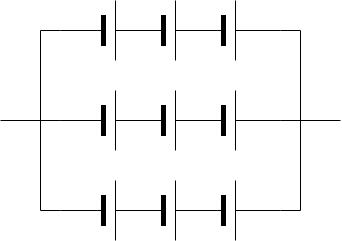
\includegraphics[width=0.5\textwidth]{chapters/images/battery_layout.png}
        \caption{Sposób połączenia baterii}
        \label{fig:battery_layout}
    \end{figure}


	\textbf{Wydajność energetyczna - TBD}

	\textbf{Responsywność - TBD}

	\textbf{Bezpieczeństwo - TBD}

	\section{Możliwe rozszerzenia}

        W ramach niniejszej pracy stworzony został prototyp rozwiązania. Niektóre planowane funkcjonalności nie zostały zaimplementowane ze względu na ograniczenia czasowe i budżetowe. Pozostawiono jednak możliwość rozbudowy systemu. Poniżej przedstawiono kilka problemów, których system w obecnym stanie nie adresuje, wraz z możliwymi rozwiązaniami.

        \subsection{Mechanizm wyjścia}

            Opisywane rozwiązanie nie obejmuje implementacji mechanizmu opuszczenia strefy chronionej systemem kontroli dostępu. W zależności od potrzeb końcowego użytkownika, możliwe rozwiązanie to montaż dodatkowego czytnika po przeciwnej stronie drzwi i połączenie go z kontrolerem wejścia w przypadku gdy wymagana jest obustronna kontrola dostępu bądź zastosowanie przycisku którego naciśnięcie powoduje zwolnienie zamka w przypadku gdy wymagana jest tylko kontrola wejścia do chronionego obszaru.

        \subsection{Obsługa większej liczby zamków}

            W celu umożliwienia obsługi przez system liczby zamków przekraczającej 1, wystarczająca byłaby modyfikacja podsystemu autoryzacji w taki sposób, aby mógł on obsługiwać równoległe żądania od klientów.

        \subsection{Wygodna konfiguracja parametrów sieci}

            W obecnej implementacji dane dostępu do sieci (nazwa sieci oraz hasło) zostały zagnieżdżone w oprogramowaniu konrolera. Zmniejsza to elastyczność konfiguracji urządzenia, wymagając jego przeprogramowania za każdym razem gdy zmianie ulegnie nazwa lub klucz dostępu do sieci.

            Możliwym rozwiązaniem tego problemu byłaby implementacja trybu konfiguracji. Tryb ten powodowałby przejście kontrolera w tryb Access Point przy zachowaniu dwóch warunków: (1) nastąpiło uruchomienie, a nie wybudzenie z trybu głębokiego uśpienia oraz (2) na określonym wejściu pojawił się stan wysoki. Przejście kontrolera w tryb Access Point umożliwiłoby udostępnienie prostego interfejsu webowego, za pomocą którego administrator systemu mógłby wprowadzić niezbędne do działania dane, takie jak nazwa sieci, hasło, a także adres IP i numer portu serwera autoryzacji. Aby zachować wysoki poziom bezpieczeństwa, komunikacja pomiędzy urządzeniem administratora i kontrolerem powinna odbywać się przy wykorzystaniu protokołu TLS.

        \subsection{Sygnalizacja stanu baterii}

            W obecnym stanie system nie implementuje mechanizmów informowania serwera o swoim stanie energetycznym.
            Sygnalizacja stanu baterii umożliwiłaby administratorowi systemu bieżące monitorowanie wszystkich zamków objętych systemem oraz szybką reakcję w przypadku, gdy baterie wymagałyby wymiany. Modyfikacja ta wymagałaby uzyskania dostępu do danych na temat naładowania baterii przez mikrokontroler oraz przesyłania ich okresowo do serwera, najlepiej w momentach, gdy jest on już wybudzony z powodu wykrycia ruchu w jego otoczeniu.

        \subsection{Obsługa kont użytkowników w podsystemie zarządzania}
            Podsystem zarządzania nie implementuje mechanizmu dostępu do zasobów, co czyni system mniej bezpiecznym. W końcowym produkcie należałoby rozszerzyć go o możliwość tworzenia kont użytkowników i przypisywania im określonych uprawnień co do odczytu i zapisu danych.

    \section{Podsumowanie}

        W ramach niniejszej pracy stworzono funkcjonalny prototyp systemu, który po odpowiednich modyfikacjach miałby szansę efektywnej pracy w odpowiednim środowisku.

        Dzięki wykorzystaniu zdalnego serwera do przeprowadzenia procesu uwierzytelniania system zapewnia większą elastyczność i łatwość zarządzania niż alternatywne systemy wykorzystujące zamki pracujące w sposób autonomiczny.

        Rozwiązanie cechuje się wygodą montażu, ponieważ nie wymaga przewodów zasilających i komunikacyjnych prowadzonych w ścianach budynków. Przy wdrażaniu rozwiązania nie jest konieczna modyfikacja istniejącej infrastruktury budynku, z wyjątkiem wymiany samych zamków. System nie wymaga żadnych dodatkowych komponentów sprzętowych poza zamkami i serwerem.

        Wydajność energetyczna podsystemu sterowania zamkiem została osiągnięta przez zarządzanie zasilaniem jego peryferiów oraz kontrolę stanu zasilania mikrokontrolera w celu minimalizacji poboru mocy i maksymalizacji czasu pracy na zasilaniu bateryjnym.

        Bezpieczeństwo systemu na wielu poziomach zapewnia wykorzystanie mechanizmów takich jak TLS w warstwie komunikacji pomiędzy zamkiem a serwerem czy szyfrowanie pamięci Flash w warstwie operacji na danych w mikroprocesorze w układzie zamka.